%!TEX root = ../thesis.tex
%*******************************************************************************
%*********************************** Second Chapter *****************************
%*******************************************************************************

\nomenclature[z-TMQ]{TMQ}{Total vertically integrated precipitation from CESM-LE.}
\nomenclature[z-PS]{PS}{Pressure at reference height of $2\si{\meter}$ from CESM-LE.}
\nomenclature[z-TREFHT]{TREFHT}{Temperature at reference hieght of $2\si{\meter}$ from CESM-LE.}
\nomenclature[z-U10]{U10}{Wind speed at height of $10\si{\meter}$ from CESM-LE.}
\nomenclature[z-CESM-LE]{CESM-LE}{Community Earth System Model - Large Ensemble.}

\chapter{Data Sets\label{cha:data}}  %Title of the Second Chapter

\ifpdf
    \graphicspath{{Chapter2/Figs/Raster/}{Chapter2/Figs/PDF/}{Chapter2/Figs/}}
\else
    \graphicspath{{Chapter2/Figs/Vector/}{Chapter2/Figs/}}
\fi

In the following chapter we describe in detail our data which we will use as a source for assessing the performance of the models described within.
We use a publicly available set of climate model simulations known as the CESM Large Ensemble (CESM-LE) data set, \citep{kay_community_2015}.
The CESM-LE data set provides a good example of EO data that is discussed in Section~\ref{sec:eo}. The data set is publicly available from \url{https://www.cesm.ucar.edu/projects/community-projects/LENS/data-sets.html}.

 \section[CESM-LE]{\label{sec:cesmle}Community Earth System Model - Large Ensemble}
 The CESM-LE data set is an extremely popular and significant data set in the climate research community.
 It was developed to enable the assessment of recent past and near future climate change in the presence of internal climate variability, \citep{kay_community_2015}.
 It does so by providing $40$ simulations of a complex climate model where each simulation is subject to the same radiative forcing scenario but initialised from a slightly perturbed atmospheric state.
 As such the forty resultant simulations present the various trajectories the model might take due to internal climate variability of the model. 
 
 The model used to run the forty member ensemble is the Community Earth System Model version 1, \citep{hurrell_community_2013}, with the Community Atmosphere model version 5, \citep{hurrell_community_2013}, as the atmospheric component.
 The model is a fully coupled climate model which consists of a model for each of land, ocean, atmosphere and sea ice components of the climate.
 These are brought together with a coupler model.
 Figure~\ref{fig:cesm} provides a simple overview as to how CESM model couples the various components.
 Such a model is capable of simulating various Land, Ocean, Atmosphere and Sea Ice variables of the climate, such as the wind speed, temperature or pressure.
 The CESM-LE produces simulations of such variables on the nominal $1\deg$ horizontal separation across the globe which induces our spatial resolution of the data.
 The ensemble produces variables at three different levels of temporal resolution between the years 1920 and 2100 for non-control simulations. The ensemble is able to produce variables at 6-hourly, daily, and monthly intervals. 
 
 \begin{figure}[htbp!] 
 	\centering    
 	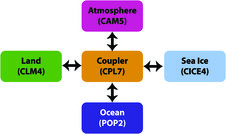
\includegraphics[width=1.0\textwidth]{cesm_components}
 	\caption[CESM component models]{The component models for the full CESM model, Figure from \citep{kay_community_2015}. The individual component models are atmospheric (CAM5), ocean (POP2), land (CLM4), Sea Ice (CICE4), and coupler (CPL7). Details of which can be found in \citep{kay_community_2015} and \citep{hurrell_community_2013}.}
 	\label{fig:cesm}
 \end{figure}

 For this body of work we use the CESM-LE data by considering the forty members as separate simulations.
 Each simulation represents a single realisation of the various climate variables generated by the model described in \citep{kay_community_2015} where the variation between realisations is coming from the internal climate variability. 
 We apply a set of preprocessing to the raw data provided by the CESM-LE model as described below. 
 
 \subsection{Preprocessing \label{sec:preprocessing}}
 The full CESM-LE data consists of a large number of climate variables on a relatively large spatial grid consisting of $192 \times 276$ locations and as such is a rather large data set. 
 The main goal in our preprocessing is to reduce the size of the data through a series of variable selection, spatial resampling, and temporal sectioning.
 We reduce the data size by considering only a subset of the full data set by selecting four variables to study from the full model which are; temperature, pressure, wind speed, and precipitation. 
 The next preprocessing step we use is a temporal cut.
 We consider only the output of the CESM-LE which occurs between December 2020 and January 2026. 
 These time points were chosen such that the length of time gave reasonable ability to capture periodic elements but that the size of the data did not become too large.
 By using monthly frequency observations and this five year time horizon we have a sixty temporal observations for each spatial grid point and for each of our four variables considered. 
 
 The final step in our preprocessing pipeline is to reduce the spatial dimension.
 To do this we resample the model simulations to a smaller spatial grid for each variable of interest.
 Resampling is achieved by averaging values of neighbouring locations until our desired resolution is achieved.
 In this case we resample until the spatial size of the data set is $64 \times 96$ which corresponds to a reduction factor of $3$ from the original CESM-LE data.
 Figure~\ref{fig:cesm_grid} shows the comparison between the full and resampled spatial observation grid over the globe due to our preprocessing step
 The figure uses the temperature variable as at January 2021 as an illustrative example. 
 Obviously using such an approach reduces the spatial resolution and thus our ability to see small scale spatial patterns.
 However, this is traded off against agility in terms of modelling due to the reduced data size.
 The reduction factor of $3$ was chosen based on this trade off.
 
 \begin{figure}[htbp!] 
 	\centering    
	\begin{subfigure}[b]{0.45\textwidth}
		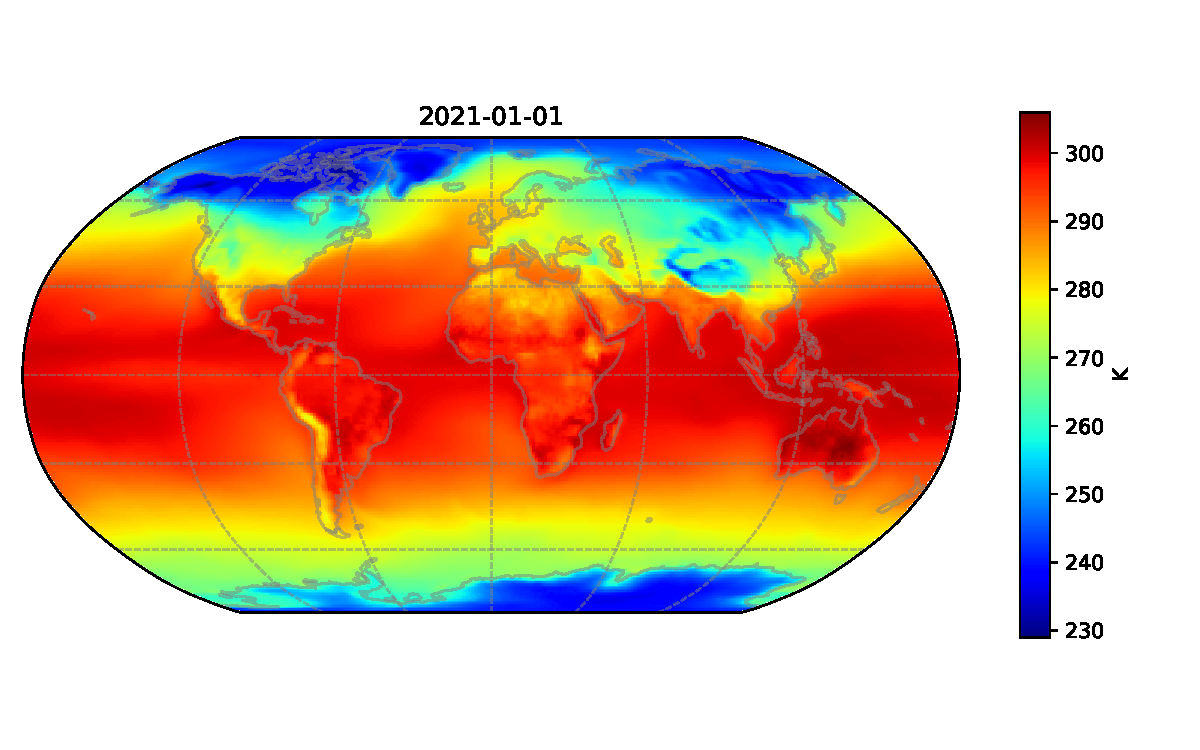
\includegraphics[width=\textwidth]{full_grid}
		\caption{Full resolution.}
		\label{fig:full_res}   
	\end{subfigure}             
	\begin{subfigure}[b]{0.45\textwidth}
		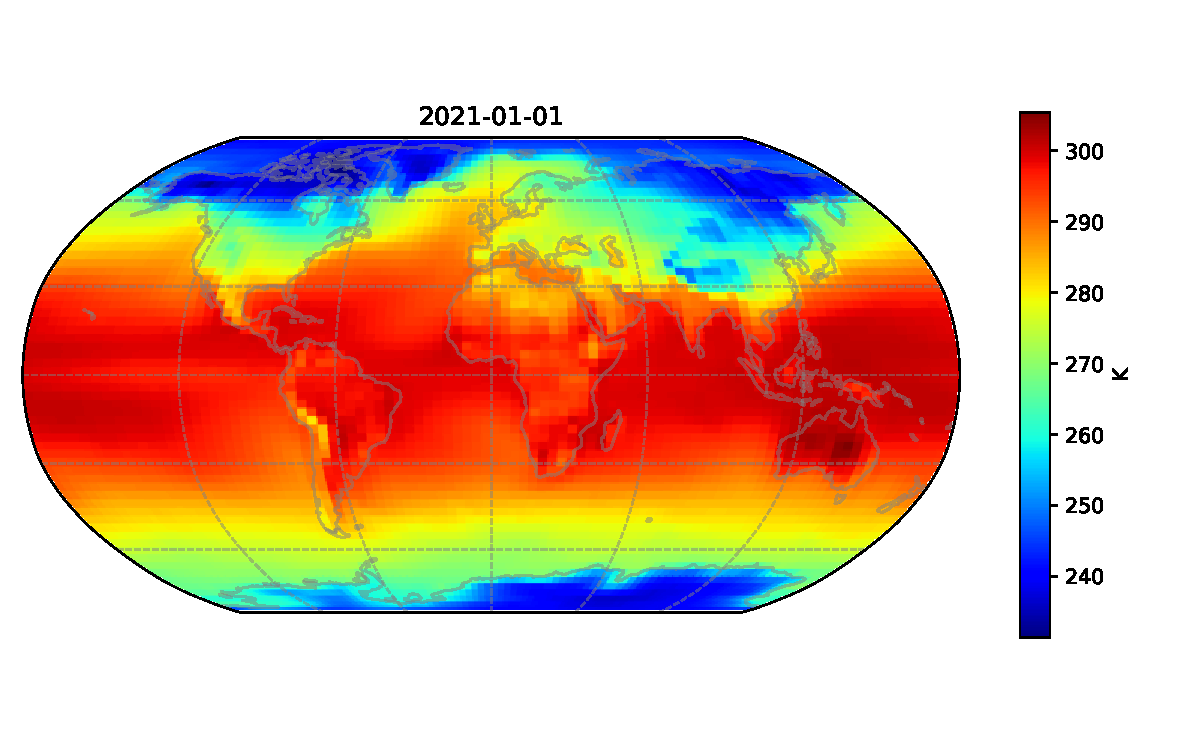
\includegraphics[width=\textwidth]{coarse_grid}
		\caption{Reduced resolution.}
		\label{fig:coarse_res}
	\end{subfigure}             
 	\caption[CESM-LE resampled spatial grid after preprocessing]{The resampled spatial grid of observation measurements across the globe. Notice the reduced spatial resolution in Figure~\ref{fig:coarse_res} compared to that in Figure~\ref{fig:full_res} due to the resampling causing some loss of fine spatial detail. Example used is the average monthly temperature in Kelvin ($\si{\kelvin}$) on January 2021.}
 	\label{fig:cesm_grid}
 \end{figure}

 \subsection{Variables \label{ssec:variables}}
 In the following section we focus our description to the four atmospheric model variables from the  CESM-LE simulations that we will use in this body of work.
 These are; pressure, temperature, precipitation, and wind speed.
 We describe each variable in detail in their respective section and throughout this work we consider each as a separate EO data set.
 We aim to show, through the use of an example time point and spatial locations, the various spatial and temporal processes that exist in each of these variables.
 These make such a data set a credible EO data set to test our proposed CPACE model on. 

\subsubsection{Precipitation \label{sssec:precip}}
The total (vertically integrated) precipitable water component abbreviated as TMQ is an atmospheric component output of the CESM-LE, \citep{kay_community_2015}.
The variable is given units of $\si{\kilogram\per\metre\squared} $ and is available monthly on the full spatial grid.
The monthly precipitation is calculated as the average over time from the  CESM-LE model six hourly output. 

We can see clearly the spatial variability of the precipitation over the globe by considering the heat map of June 2021 monthly precipitation for a single simulation; which is shown in Figure~\ref{fig:precip_june}. 
As one would expect there is clear spatial correlation.
For example, the tropics observe large amounts of precipitation whereas desert regions observe little. 
We can also see some subtler differences in the spatial correlation structure. 
Figure~\ref{fig:precip_june} shows that bands of precipitation are evident over the globe.
This indicates that precipitation is much more correlated over lines of latitude than lines of longitude. 
This may be an indicator of spatial anisotropy in the generating process.
There is also a case of observing more complex, possibly non stationary, spatial processes as the correlation structure seems different between say North America and Indonesia. 
We can similarly observe clear temporal correlations in the precipitation variable of the CESM model.
In particular, Figure~\ref{fig:precip_temp} shows the time series of two locations; the United Kingdom (UK) and Colombia.
Each exhibit clear periodic signals as wet seasons and dry seasons repeat each year.
However, we can see a clear level difference between the UK and Colombia precipitation as well as differences in the range of precipitation.
This highlights the fact that not only do we have temporal correlation but this correlation is dependent on location. 

\begin{figure}[htbp!] 
	\centering
	\begin{subfigure}[b]{0.45\textwidth}
		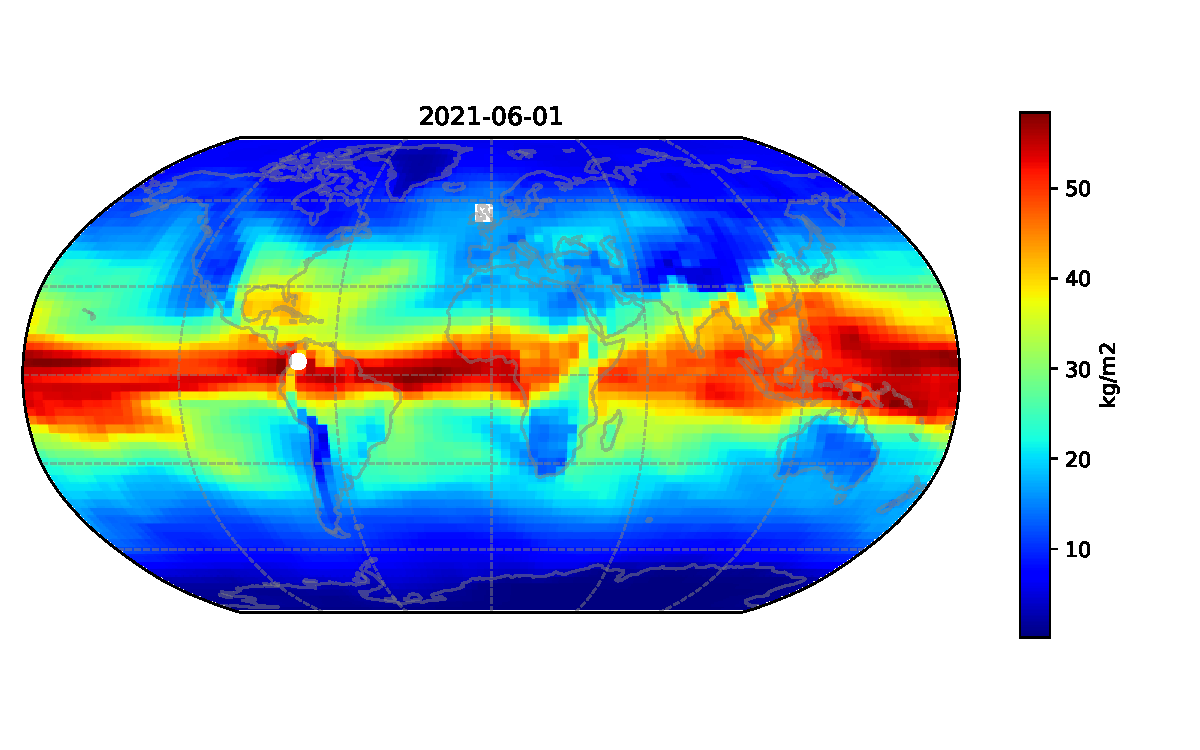
\includegraphics[width=\textwidth]{TMQ_example}
		\caption{TMQ as at June 2021.}
		\label{fig:precip_june}   
	\end{subfigure}             
	\begin{subfigure}[b]{0.45\textwidth}
		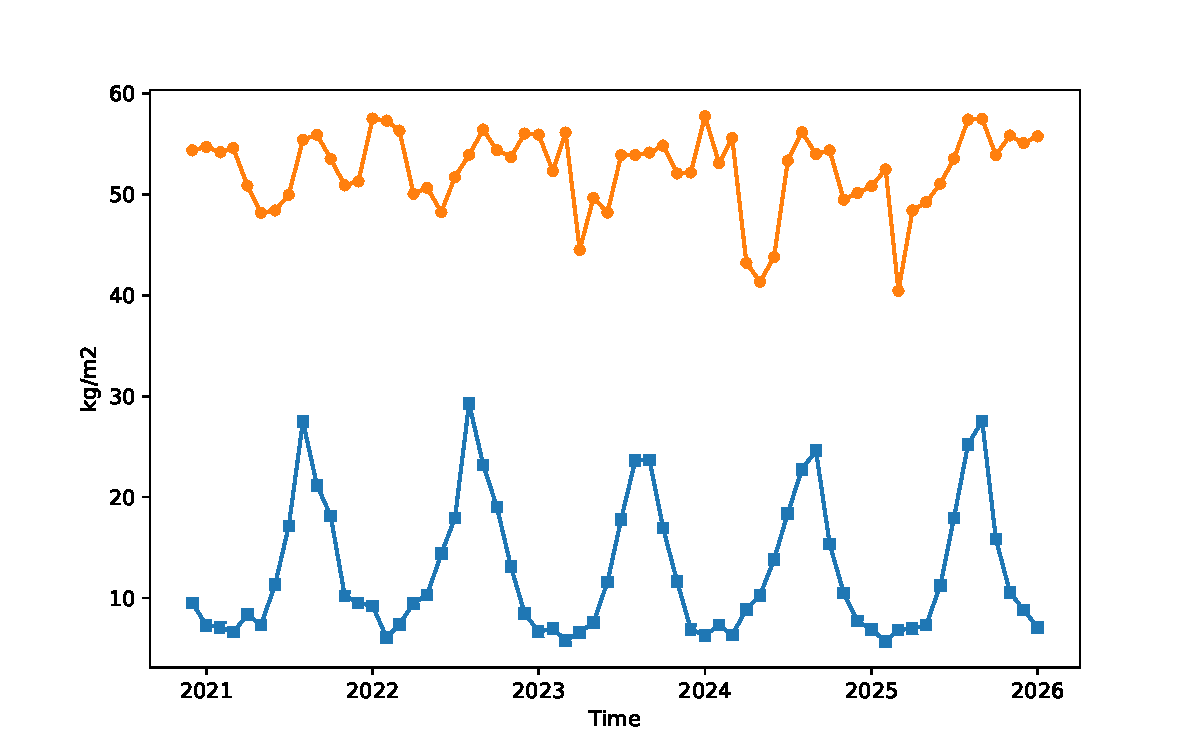
\includegraphics[width=\textwidth]{TMQ_example_temp}
		\caption{TMQ over time.}
		\label{fig:precip_temp}
	\end{subfigure}             
	\caption[Overview of Precipitation variable]{Overview of the monthly average precipitation variable (TMQ) from CESM-LE ensemble member 1. Figure~\ref{fig:precip_june} highlights the spatial correlation present while Figure~\ref{fig:precip_temp} highlights the temporal correlation at two distinct locations; namely Colombia and the United Kingdom. The orange circle and blue square markers mark these respectively on Figure~\ref{fig:precip_temp} with the white markers highlighting their locations in Figure~\ref{fig:precip_june}. Note the level difference in temporal correlation structure between the two locations, indicative of a spatio-temporal correlation process occurring.}
	\label{fig:precip_overview}
\end{figure}

\subsubsection{Pressure \label{sssec:pressure}}
The surface pressure variable abbreviated as PS is another atmospheric component output of the CESM-LE, \citep{kay_community_2015}.
The component is given in Pascals ($\si{\pascal}$) and represents the surface pressure at a height of $2\si{\meter}$. It is available monthly on the full spatial grid and the monthly average is calculated as the average over time from the CESM-LE model six hourly output.

Figure~\ref{fig:pressure_overview} gives a brief insight to this variable. 
We can see the spatial correlation structure of pressure over the globe in Figure~\ref{fig:pressure_june}.
One can clearly see areas of high and low pressure.
For example, there is a significant difference between the low pressure zone over Antarctica and high pressure zone over Australia. 
It is interesting to note that we see a clear difference in the smooth structure over sea and a rougher structure over land variables. 
This again might motivate that a non stationary spatial process is driving such a variable.
Considering the temporal variation displayed for Colombia and the UK in Figure~\ref{fig:pressure_temp}; we can see definite structure over time, albeit different for each location.
The UK exhibits much more variation in pressure than Colombia, however both do exhibit temporal correlation. 
Again, similar to the precipitation variable discussed in Section~\ref{sssec:precip}, this might suggest that modelling such a variable will need to consider both spatial and temporal correlations in conjunction with each other.

\begin{figure}[htbp!] 
	\centering
	\begin{subfigure}[b]{0.45\textwidth}
		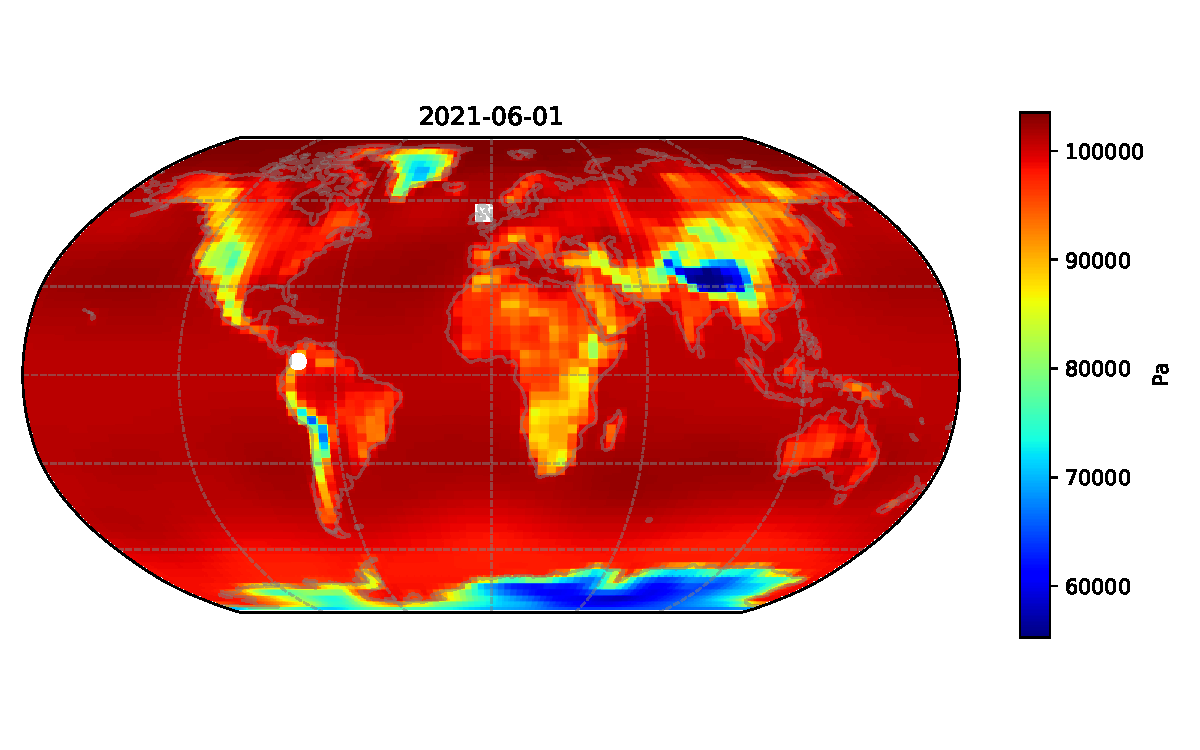
\includegraphics[width=\textwidth]{PS_example}
		\caption{PS as at June 2021.}
		\label{fig:pressure_june}   
	\end{subfigure}             
	\begin{subfigure}[b]{0.45\textwidth}
		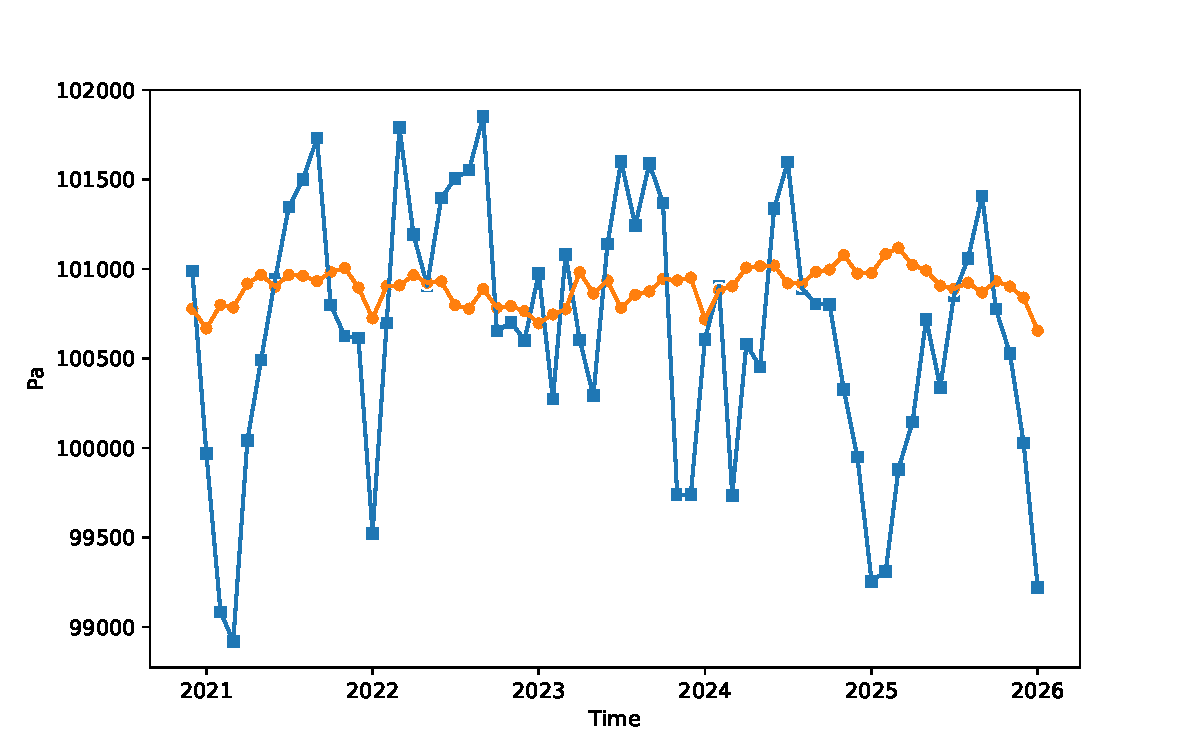
\includegraphics[width=\textwidth]{PS_example_temp}
		\caption{PS  over time.}
		\label{fig:pressure_temp}
	\end{subfigure}             
	\caption[Overview of Pressure variable]{Overview of the monthly average pressure variable from CESM-LE ensemble member 1. Figure~\ref{fig:pressure_june} highlights the spatial correlation present while Figure~\ref{fig:pressure_temp} highlights the temporal correlation at two distinct locations; namely Colombia and the United Kingdom. The orange circle and blue square markers mark these respectively on Figure~\ref{fig:pressure_temp} with the white markers highlighting their locations in Figure~\ref{fig:pressure_june}. Notice the stark difference between the time series variance in the UK and Colombia.}
	\label{fig:pressure_overview}
\end{figure}

\subsubsection{Temperature \label{sssec:temp}}
The temperature variable abbreviated to TREFHT is an atmospheric component output of the CESM-LE, \citep{kay_community_2015}.
The variable refers to the average temperature in Kelvin ($\si{\kelvin}$) at the model reference height which is $2\si{\meter}$ above sea level.
The average is available monthly with said average being calculated from the model six hourly output over the month.

Quite clearly the temperature exhibits spatial correlation across the globe and periodic signals through time the seasons unfold.
Figures~\ref{fig:temp_june},~\ref{fig:temp_temp} highlight this for the spatial and temporal correlation respectively.
Clearly the temperature at June increases as we move closer to the equator and decreases at the poles. 
Similarly to the precipitation, we observe that the spatial correlation structure is clearly anisotropic. 
Correlation is much more pronounced over longitude than latitude. 
Looking more deeply at Figure~\ref{fig:temp_overview} we can observe more complex correlation structures, as mentioned in Section~\ref{sec:eo}. 
For example, Asia exhibits a localised area of low temperature right next to an area of relatively high temperature. 
This is very different to the extremely smooth variation that we see over the larger oceans such as the Atlantic. 
Again similar to the previous variables, this is an indication that there may be a non-stationary spatial process helping to drive this variable.

Figure~\ref{fig:temp_temp} gives an insight into the temporal correlation structure in the variable for two locations; namely Colombia and the UK. 
There is strong evidence of a periodic signal driving both but clearly there is a level shift and change in amplitude for the two locations. 
This is again similar to the precipitation variable discussed in Section~\ref{sssec:precip} and motivates the idea that there is a clear spatio-temporal process driving the variable rather than just either temporal or spatial process.

\begin{figure}[htbp!] 
	\centering
	\begin{subfigure}[b]{0.45\textwidth}
		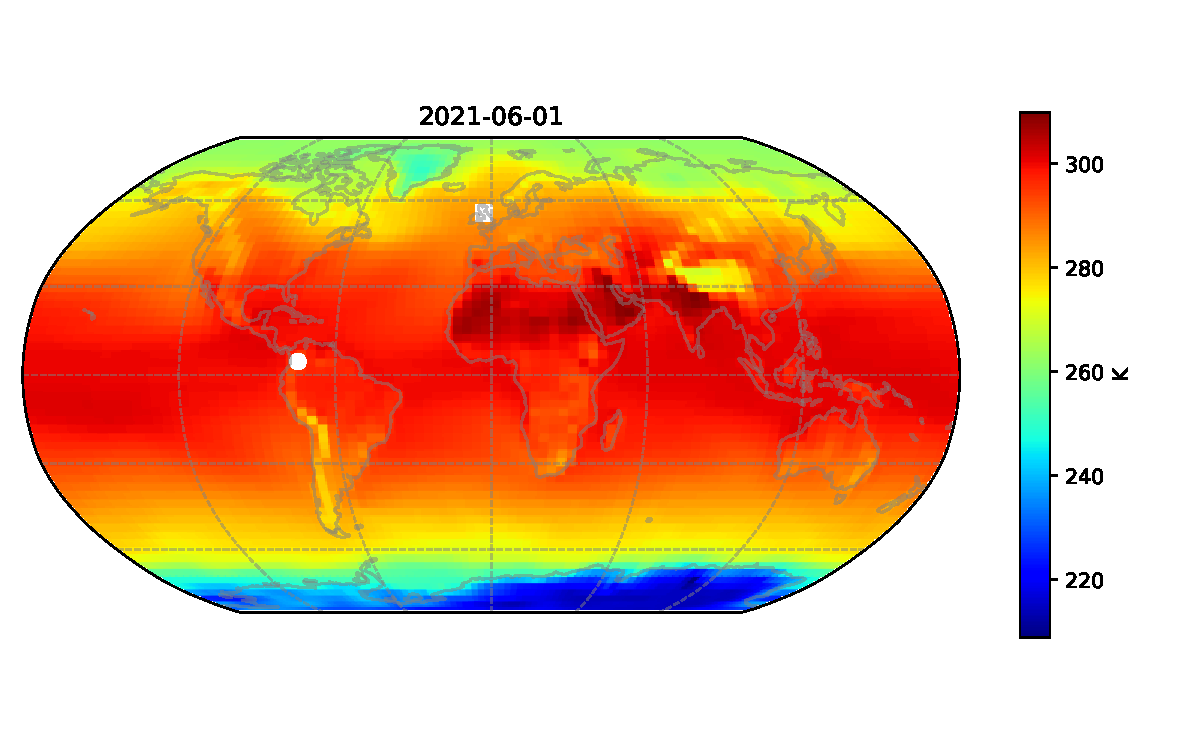
\includegraphics[width=\textwidth]{TREFHT_example}
		\caption{TREFHT as at June 2021.}
		\label{fig:temp_june}   
	\end{subfigure}             
	\begin{subfigure}[b]{0.45\textwidth}
		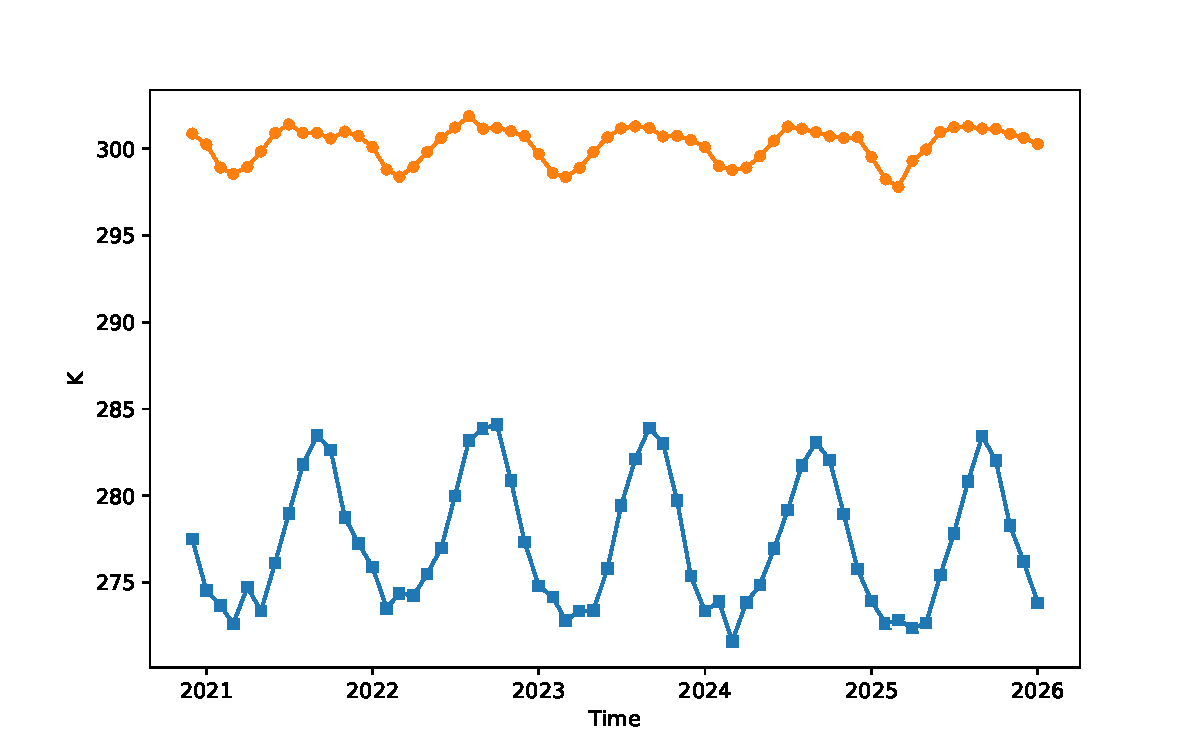
\includegraphics[width=\textwidth]{TREFHT_example_temp}
		\caption{TREFHT  over time.}
		\label{fig:temp_temp}
	\end{subfigure}             
	\caption[Overview of Temperature variable]{Overview of the monthly average temperature variable from CESM-LE ensemble member 1. Figure~\ref{fig:temp_june} highlights the spatial correlation present while Figure~\ref{fig:temp_temp} highlights the temporal correlation at two distinct locations; namely Colombia and the UK. The orange circle and blue square markers mark these respectively on Figure~\ref{fig:temp_temp} with the white markers highlighting their locations in Figure~\ref{fig:temp_june}.}
	\label{fig:temp_overview}
\end{figure}

\subsubsection{Wind speed \label{sssec:wind}}
The wind speed variable  abbreviated to U10 is another atmospheric component output of the CESM-LE model.
The variable refers to the average wind speed in $\si{\meter\per\second}$ at a height of $10\si{\meter}$ above sea level.
Again the variable is available on the full spatial grid and is available as a monthly average over time.

We visualise the spatial correlation of the variable in Figure~\ref{fig:wind_june} by considering a snap shot of the monthly average wind speed in June 2021.
We can see, in contrast to the previous three variables, that this has a much rougher spatial correlation structure over the sea. 
In fact it is interesting to observe the distinct difference in variability over the sea compared to that over the land. 
This may suggest that we have two types of correlation structure existing for this variable, one for the land and one for the sea. 
In this case the model for the whole variable will clearly need to include a non-stationary spatial component to capture such a phenomena.
Wind speed, like the other studied model variables, also exhibits temporal correlation. 
This is illustrated for the usual two locations, Colombia and the UK, in Figure~\ref{fig:wind_temp}. 
The temporal correlation is much less pronounced for this variable than compared to the others. 
Visually there is perhaps evidence for a periodic signal for the UK location. 
However, yet again we do see a clear level shift between the two location. 
This again suggests that the spatial coordinate clearly impacts the observed function of wind speed over time.
Similar to the other variables this suggests a model which includes both space and time as drivers for the process.

\begin{figure}[htbp!] 
	\centering
	\begin{subfigure}[b]{0.45\textwidth}
		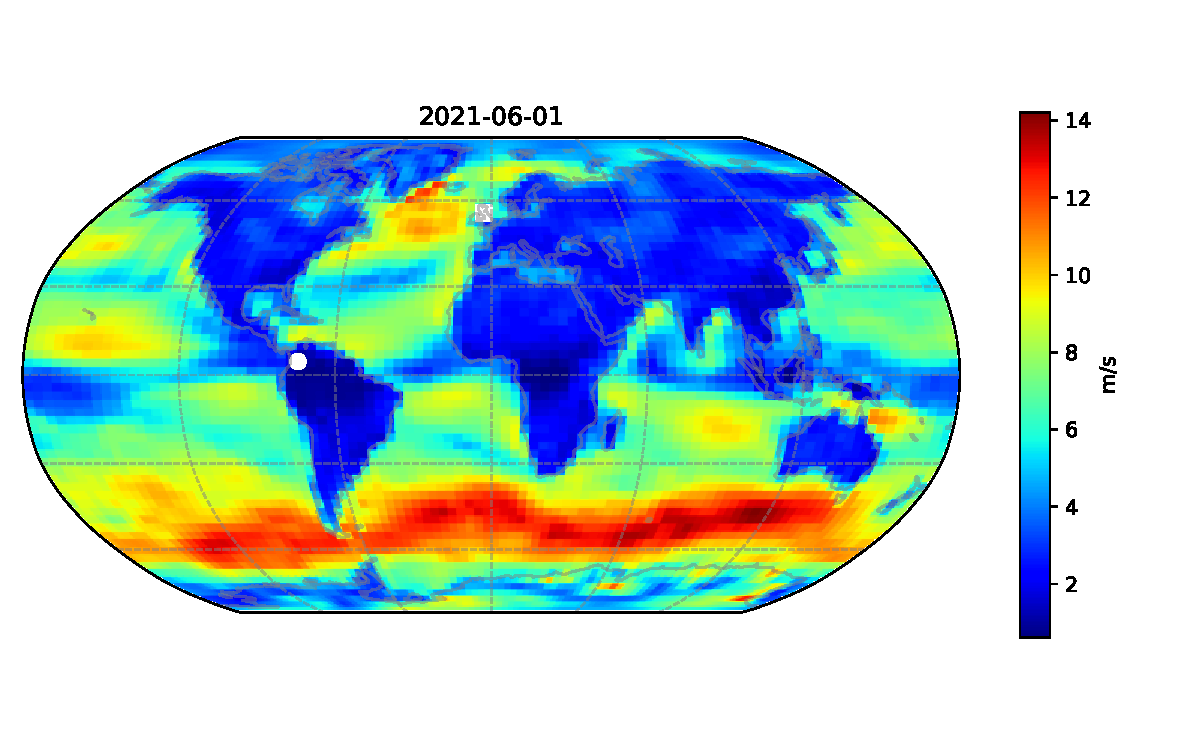
\includegraphics[width=\textwidth]{U10_example}
		\caption{U10 as at June 2021.}
		\label{fig:wind_june}   
	\end{subfigure}             
	\begin{subfigure}[b]{0.45\textwidth}
		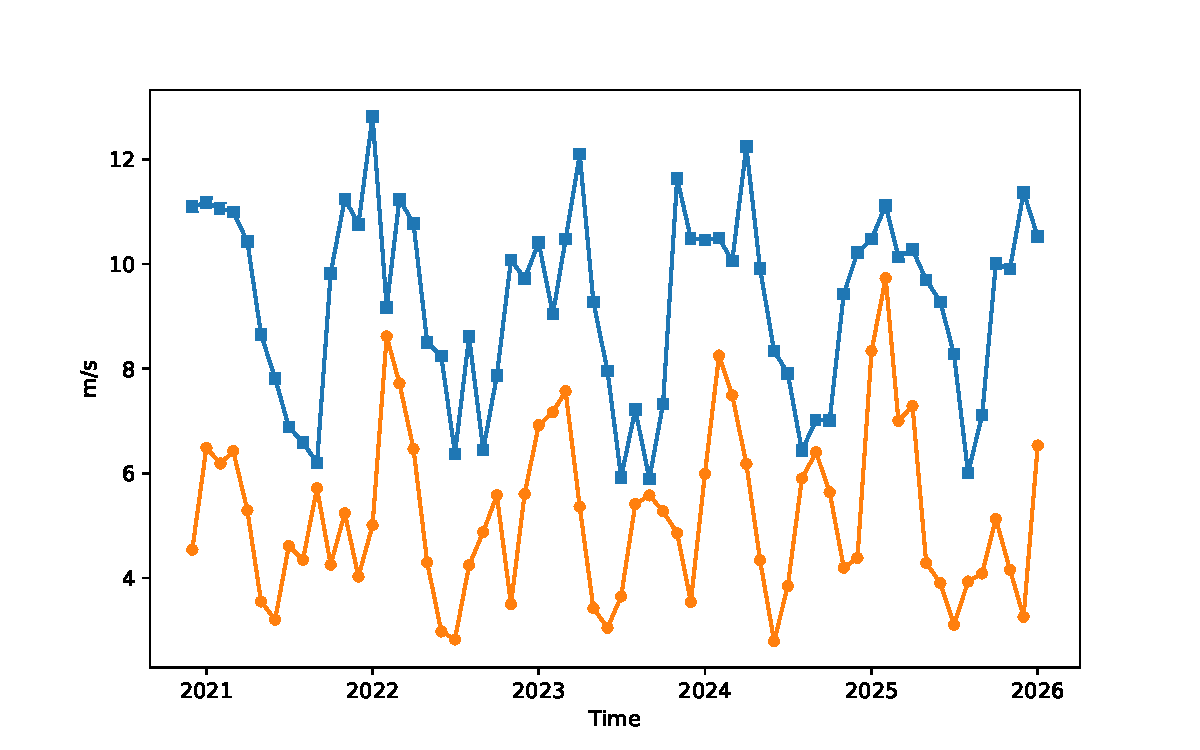
\includegraphics[width=\textwidth]{U10_example_temp}
		\caption{U10 over time.}
		\label{fig:wind_temp}
	\end{subfigure}             
	\caption[Overview of Wind variable]{Overview of the monthly average wind variable from CESM-LE ensemble member 1. Figure~\ref{fig:wind_june} highlights the spatial correlation present while Figure~\ref{fig:wind_temp} highlights the temporal correlation at two distinct locations; namely Colombia and the UK. The orange circle and blue square markers mark these respectively on Figure~\ref{fig:wind_temp} with the white markers highlighting their locations in Figure~\ref{fig:wind_june}.}
	\label{fig:wind_overview}
\end{figure}

\subsection{Replications}
For each variable discussed in Section~\ref{ssec:variables} the CESM-LE data provides $40$ replications; one from each ensemble member.
We have illustrated the spatial and temporal correlations in the four variables in the Figures~\ref{fig:precip_overview},~\ref{fig:pressure_overview},~\ref{fig:temp_overview}, and~\ref{fig:wind_overview} for a single simulation.
However we also have variability between replications and it is useful to illustrate this as it may provide insight into where we may expect difficulty in modelling.
It is important that any model developed for such data should be able to account for this variability in the data generating process.
Figure~\ref{fig:std_overview} displays a snap shot of the standard deviation of the respective variables in June 2021.

\begin{figure}[htbp!] 
	\centering
	\begin{subfigure}[b]{0.45\textwidth}
		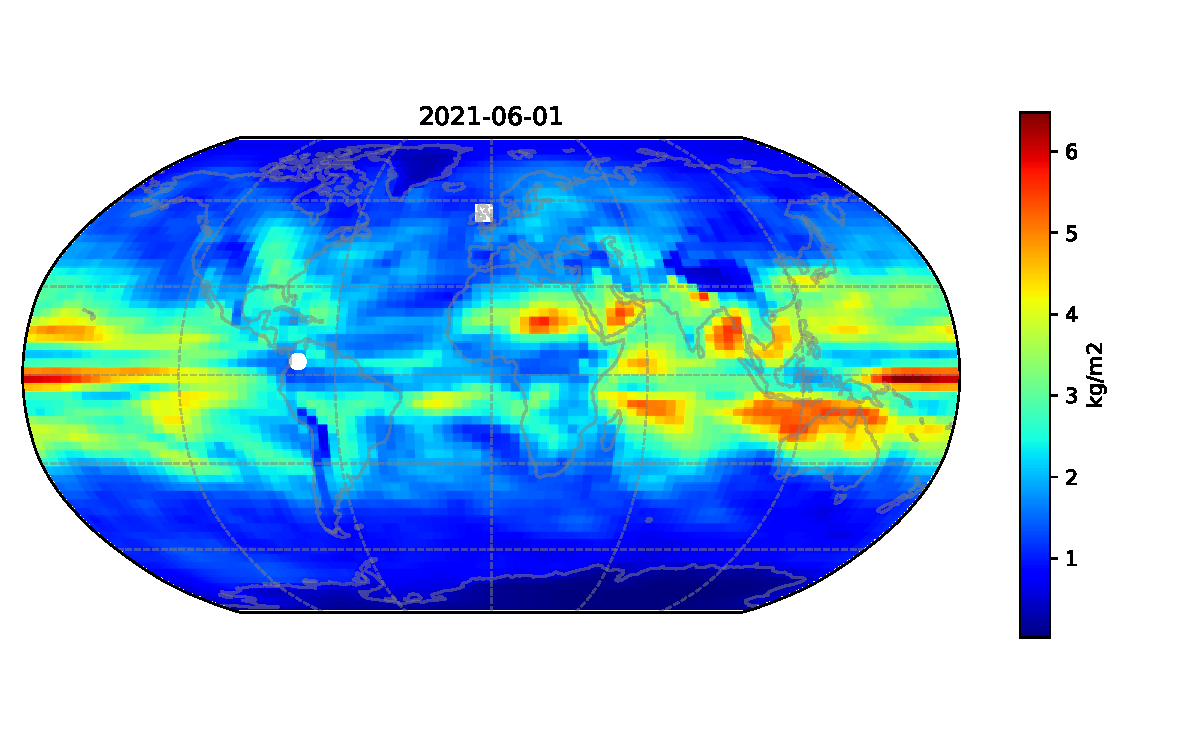
\includegraphics[width=\textwidth]{TMQ_std}
		\caption{TMQ.}
		\label{fig:std_precip_june}   
	\end{subfigure}             
	\begin{subfigure}[b]{0.45\textwidth}
		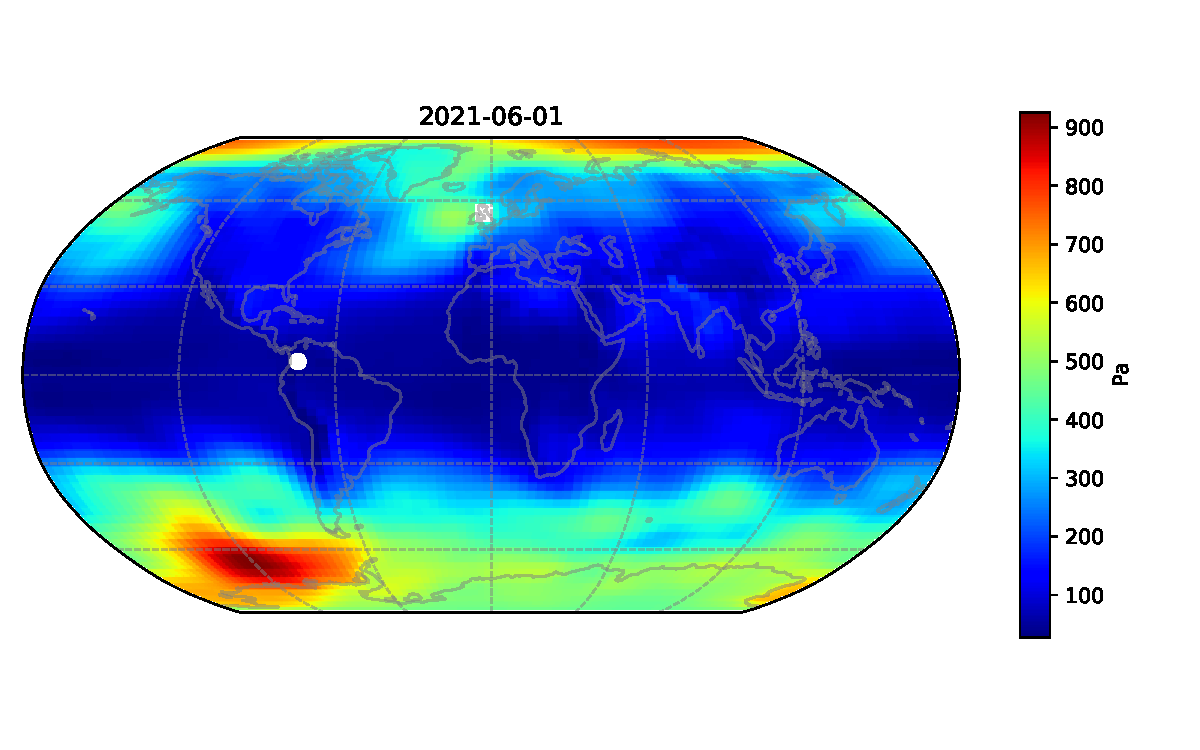
\includegraphics[width=\textwidth]{PS_std}
		\caption{PS.}
		\label{fig:std_pressure_june}
	\end{subfigure}             
	\hfill
		\begin{subfigure}[b]{0.45\textwidth}
		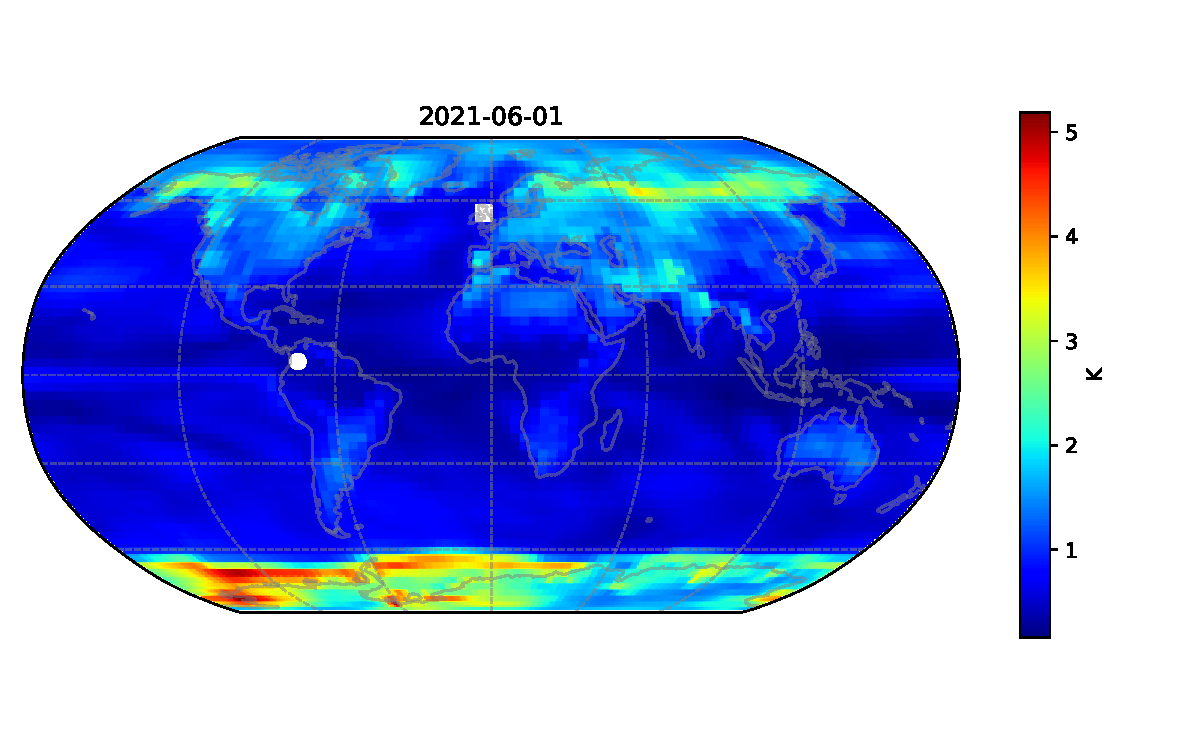
\includegraphics[width=\textwidth]{TREFHT_std}
		\caption{TREFHT.}
		\label{fig:std_temp_june}   
	\end{subfigure}             
	\begin{subfigure}[b]{0.45\textwidth}
		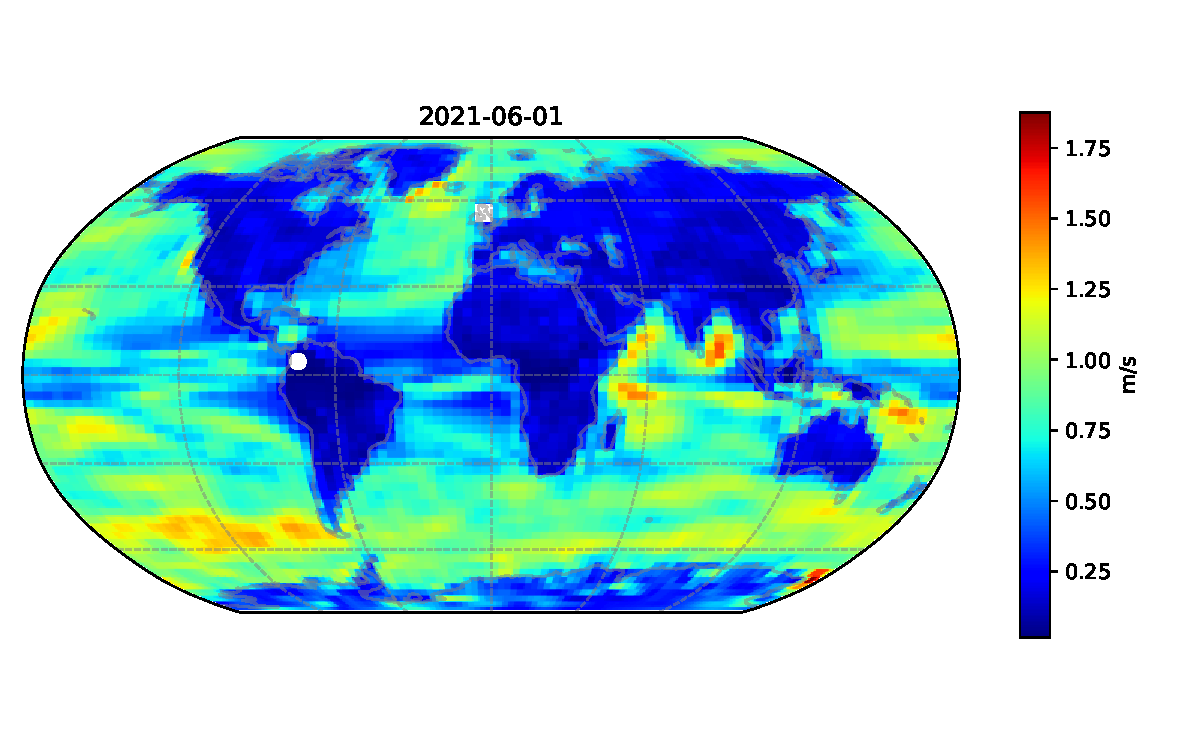
\includegraphics[width=\textwidth]{U10_std}
		\caption{U10.}
		\label{fig:std_wind_june}
	\end{subfigure}             
	\caption[Spatial overview of variability of Precipitation, Pressure, Temperature, and Wind speed.]{ Standard deviation of the four variables considered at June 2021 for the $40$ replications present in the CESM-LE data set. The locations of the UK and Colombia are shown by the white square and circle markers respectively. These points are used as examples in Figure~\ref{fig:std_overview_temp}. }
	\label{fig:std_overview}
\end{figure}

Figure~\ref{fig:std_overview} gives an indication of how drastically each simulation differs for each variable.
We would like to propose a model that can accommodate all the different scenarios presented in the various replications. 
Thus our model must be able to adapt to the regions of high standard deviation. 
From Figure~\ref{fig:std_precip_june} we can see that each simulation varies significantly in the tropics, but mostly around Indonesia.
As such we might be particularly interested in our model performance in this area for the precipitation variable.
For the pressure variable there is an increase in standard deviation for the poles and particularly to the south west of Antarctica, see Figure\ref{fig:std_pressure_june}.
There is a similar result for the temperature variable in Figure~\ref{fig:std_temp_june}.
Therefore we will be interested in model performance in this area for these variables.
The wind speed variable has many more localised areas with high variance from replications.
For example, the localised high variance of the coast of India and eastern Africa.  
These may pose a significant challenge to accommodate in a model for this variable.

Similar to the spatial variability in replications we can consider the variability over time.
Figure~\ref{fig:std_overview_temp} highlights this variation over the $40$ replications from the CESM-LE data set. 

\begin{figure}[htbp!] 
	\centering
	\begin{subfigure}[b]{0.45\textwidth}
		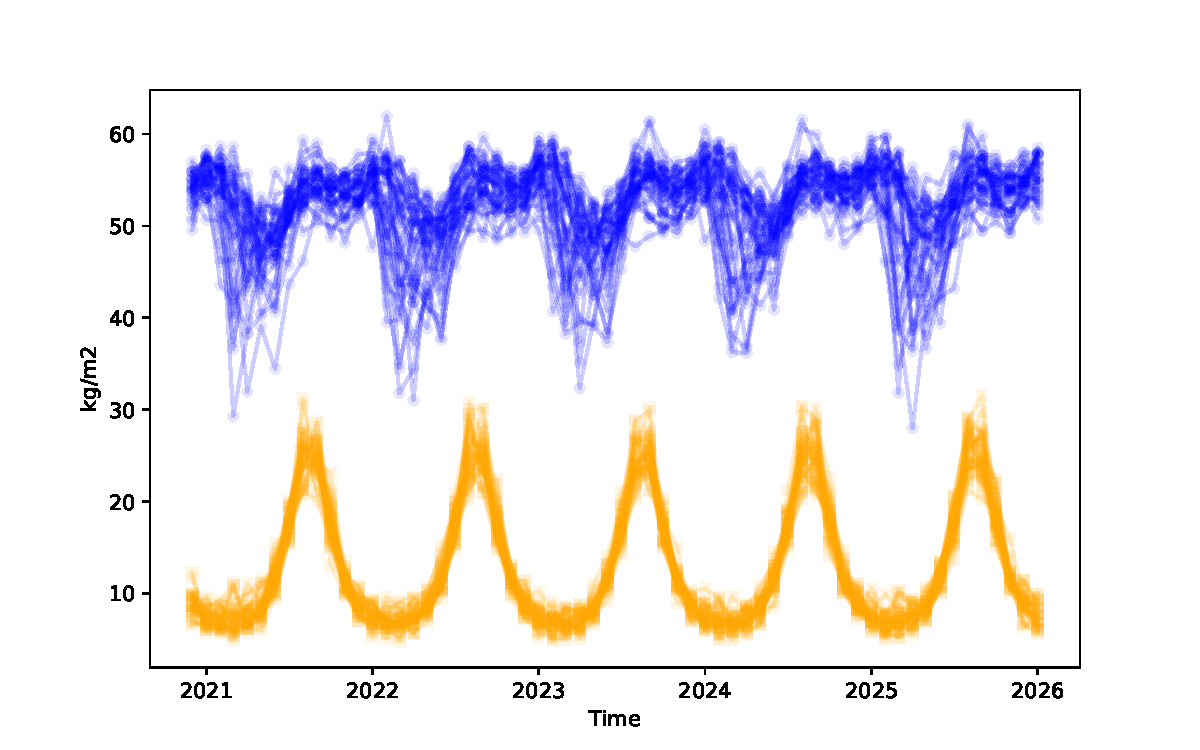
\includegraphics[width=\textwidth]{TMQ_std_temp}
		\caption{TMQ.}
		\label{fig:std_precip_temp}   
	\end{subfigure}             
	\begin{subfigure}[b]{0.45\textwidth}
		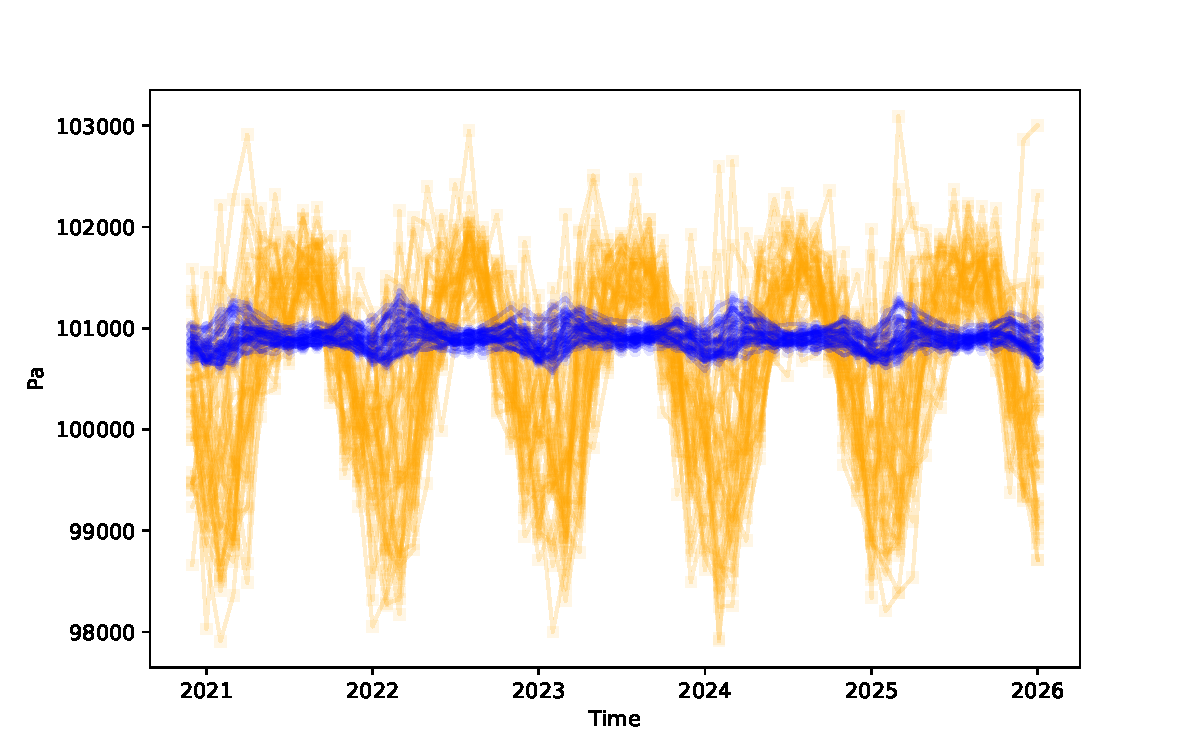
\includegraphics[width=\textwidth]{PS_std_temp}
		\caption{PS.}
		\label{fig:std_pressure_temp}
	\end{subfigure}             
	\hfill
	\begin{subfigure}[b]{0.45\textwidth}
		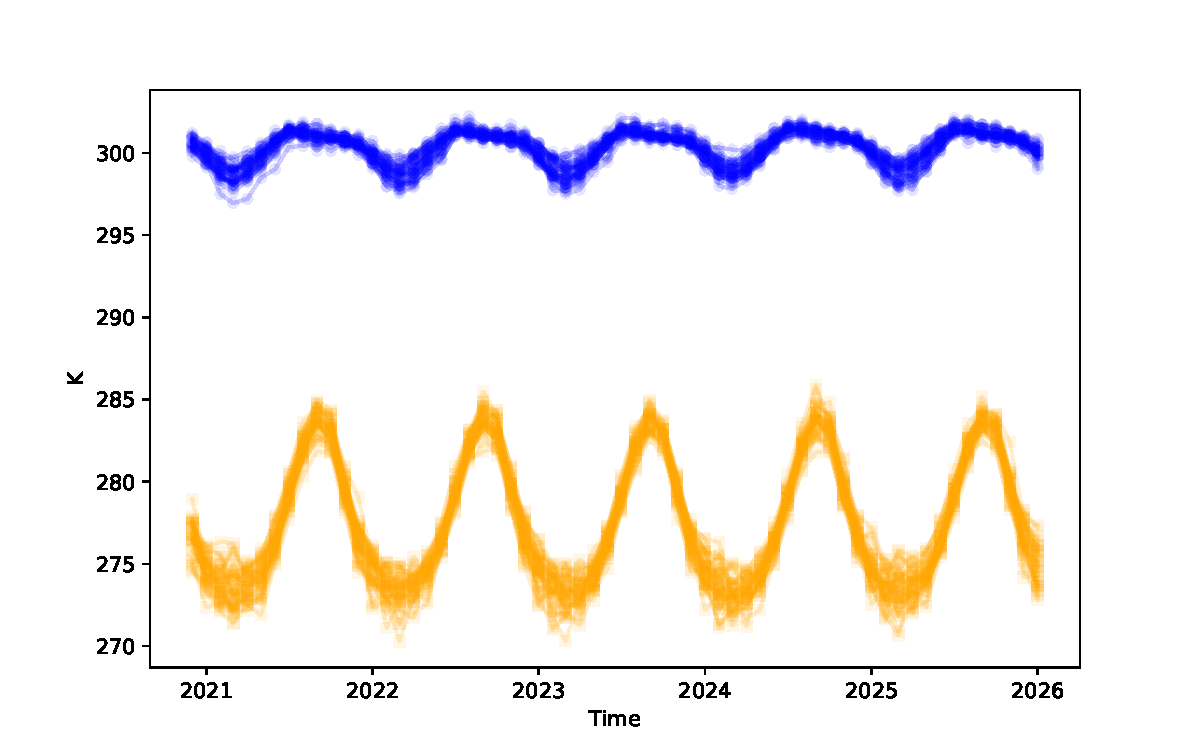
\includegraphics[width=\textwidth]{TREFHT_std_temp}
		\caption{TREFHT.}
		\label{fig:std_temp_temp}   
	\end{subfigure}             
	\begin{subfigure}[b]{0.45\textwidth}
		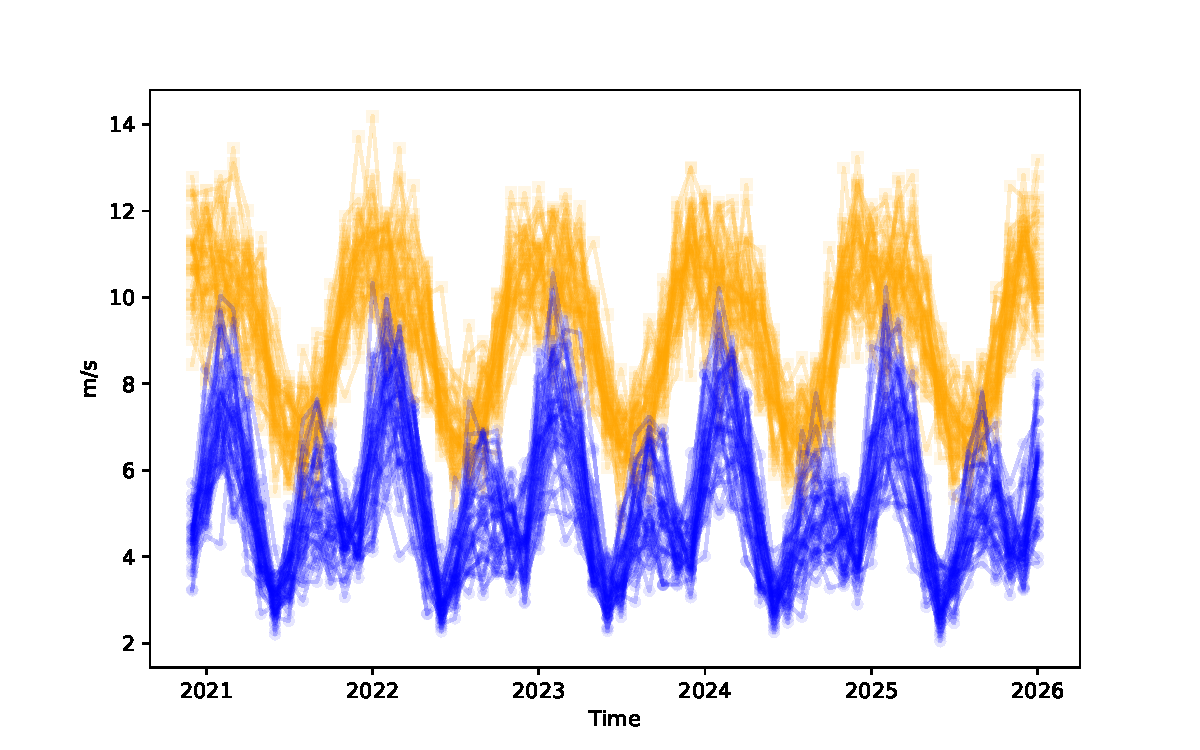
\includegraphics[width=\textwidth]{U10_std_temp}
		\caption{U10.}
		\label{fig:std_wind_temp}
	\end{subfigure}             
	\caption[Temporal overview of variability of Precipitation, Pressure, Temperature, and Wind speed.]{ Four variables over observation period December 2020 to January 2026 for the $40$ replications present in the CESM-LE data set at two locations; namely Colombia and UK. These are represented by the blue and orange colours respectively.}
	\label{fig:std_overview_temp}
\end{figure}

We can see clearly from Figure~\ref{fig:std_temp_temp} that the temperature variable function over time shows little variation between replications. 
However, variability does tend to increase in the troughs of these functions. 
Such a phenomena is more pronounced for the Colombia location. 
It may be interesting to assess performance of proposed models of the temperature variable with regard to this.
The precipitation functions vary differently for the Colombia and UK locations.
From the UK time series we see that although variability is high we can observe a periodic signal. 
It may be interesting to assess whether any model for this variable is able to pick up such a periodic signal, given that a single simulation may not show great periodicity.
Pressure similarly exhibits very different function variability between locations, with the Colombia functions showing large changes in pressure compared to the changes observed between replications at the UK location. 
Again this indicates that there is a clear spatial component to the process driving such replications. 

The above illustration of variability in replications gives an indication about the difficulties that any model must overcome to describe such variables and gives testament to the use of such a data set to test our proposed model for EO data.






